% !TEX root = ../main.tex
\chapter{Experiments and results}
In this chapter will be outlined the experimentation phase of the project.
The experimentation has been divided in two types. Since the core of the project is the semantic graph compiled through the KITT reasoner and that
\section{Reasoner performance}
For the sake of performance evaluation KITT has been deployed on a local liberty webserver, simulating the cloud based running environment of real deployments.
The performances have been evaluated in respect to the two classical measures, time and space requirements. Since real case scenarios for commercial buildings have considerably larger dimensions than the examples presented in previous chapter and that deployment data of real case wasn't available due to privacy reasons, in order to run a simulation that likely reflect real world data, the following route has been taken.
A given architecture, representing a floor of a building, has been repeated over and over until reaching the complexity of a two hundred storeys building, each of which is comprised of up to a hundred rooms. For comparison, the tallest building in the world, as of 2018, is the Burj Khalifa in Dubai with 163 storeys. From \autoref{fig:experiment_single} it can be seen the structure of the first synthetic example of the test building. Every room is equipped with four Points: a temperature sensor, an occupancy sensor, a cooling valve command and a heating valve command. The rooms are located to the side of a corridor and are adjacent up to by two. This configurations represent a floor. Floors are then stacked one upon the other to form the final building. The outside environment is supposed to monitored by a temperature sensor and an illumination sensor.
\begin{figure}
  \centering
  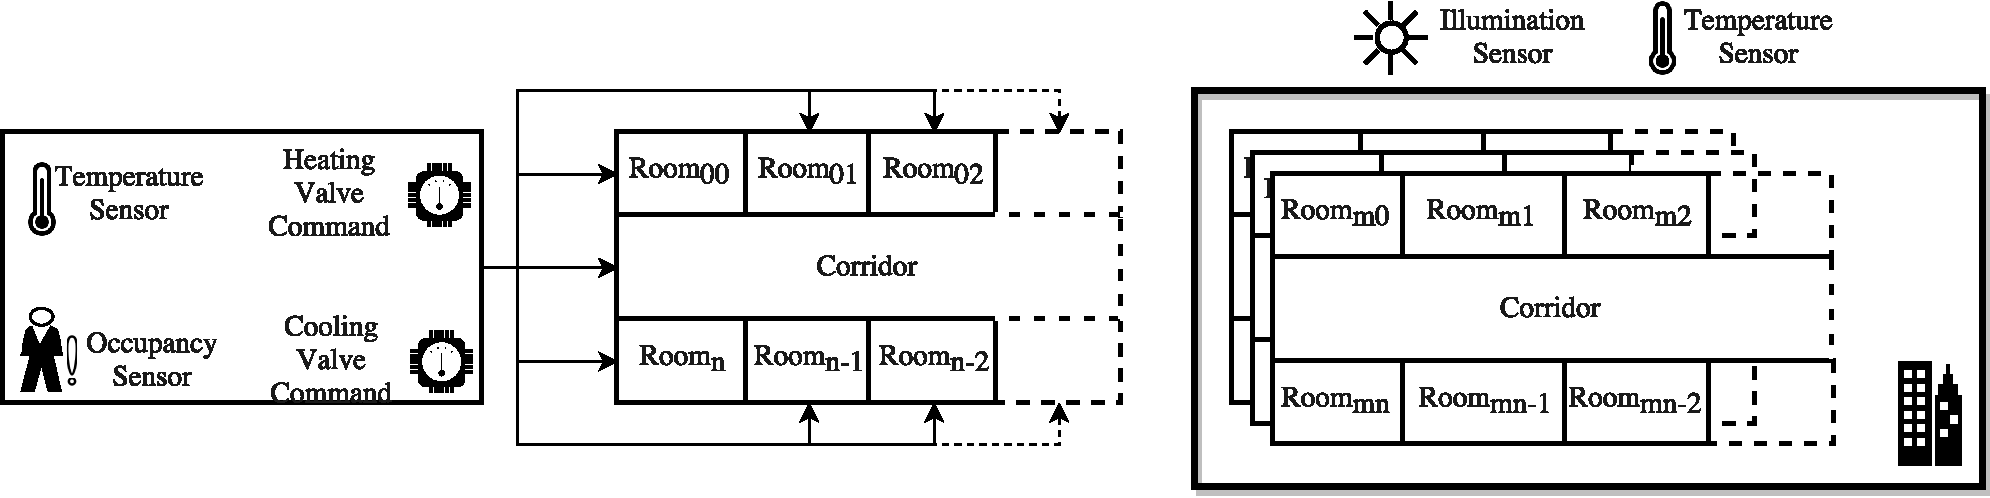
\includegraphics[width=\textwidth]{experiment_simple.pdf}
  \caption{Construction of experiment data}
  \label{fig:experiment_single}
\end{figure}
A more complex example building is derived following the same schema as above, just providing fifteen points per room and four sensors monitoring the outside environment.
Given these configurations a full stack of reasoning rules are executed so that a physical model can be derived.
\begin{table}
\centering
\caption{Performance test result for the simple model}
\label{tab:perf_simple}
\begin{adjustbox}{max width=\textwidth}
\begin{tabular}{lll|llll|llll}
\textbf{Floors} & \textbf{Rooms} & \specialcell{\textbf{No.}\\\textbf{Sensors}} & \textbf{Vertexes} & \textbf{Edges} & \specialcell{\textbf{Vertexes}\\\textbf{reasoning}} & \specialcell{\textbf{Edges}\\\textbf{reasoning}} & \specialcell{\textbf{Memory}\\\textbf{create}\\\textbf{{[}MB{]}}} & \specialcell{\textbf{Memory}\\\textbf{reasoning}\\\textbf{{[}MB{]}}} & \specialcell{\textbf{Time}\\\textbf{create}\\\textbf{{[}ms{]}}} & \specialcell{\textbf{Time}\\\textbf{reasoning}\\\textbf{{[}ms{]}}} \\\hline
1 & 1 & 10 & 123 & 381 & 143 & 477 & 8 & 54 & 16 & 95 \\
1 & 10 & 46 & 168 & 588 & 251 & 1008 & 10 & 98 & 18 & 166 \\
1 & 100 & 406 & 618 & 2658 & 1331 & 6318 & 47 & 228 & 156 & 2047 \\
10 & 10 & 82 & 672 & 2973 & 1448 & 7011 & 53 & 151 & 186 & 2587 \\
10 & 100 & 442 & 5172 & 24483 & 12248 & 61731 & 169 & 300 & 15850 & 256934 \\
20 & 100 & 482 & 10232 & 48733 & 24496 & 48733 & 62 & 284 & 73692 & 1352861 \\
50 & 100 & 602 & 25412 & 121483 & 60768 & 308011 & 143 & 267 & 492255 & 12631754 \\
80 & 100 & 722 & 40592 & 194233 & 97158 & 492721 & 261 & 416 & 1312923 & 34668894 \\
100 & 100 & 802 & 50712 & 242733 & 121418 & 615861 & 194 & 510 & 2172877 & 54904640 \\
200 & 100 & 1202 & 101312 & 485233 & 242718 & 1231561 & 922 & 1014 & 8742782 & 225609628
\end{tabular}
\end{adjustbox}
\end{table}
\begin{table}
\centering
\caption{Performance test result for the complex model}
\label{tab:perf_complex}
\begin{adjustbox}{max width=\textwidth}
\begin{tabular}{lll|llll|llll}
\textbf{Floors} & \textbf{Rooms} & \specialcell{\textbf{No.}\\\textbf{Sensors}} & \textbf{Vertexes} & \textbf{Edges} & \specialcell{\textbf{Vertexes}\\\textbf{reasoning}} & \specialcell{\textbf{Edges}\\\textbf{reasoning}} & \specialcell{\textbf{Memory}\\\textbf{create}\\\textbf{{[}MB{]}}} & \specialcell{\textbf{Memory}\\\textbf{reasoning}\\\textbf{{[}MB{]}}} & \specialcell{\textbf{Time}\\\textbf{create}\\\textbf{{[}ms{]}}} & \specialcell{\textbf{Time}\\\textbf{reasoning}\\\textbf{{[}ms{]}}} \\\hline
1 & 1 & 34 & 147 & 477 & 187 & 653 & 8 & 122 & 20 & 240 \\
1 & 10 & 169 & 291 & 1080 & 475 & 1904 & 10 & 76 & 42 & 397 \\
1 & 100 & 1519 & 1731 & 7110 & 3355 & 14414 & 47 & 268 & 713 & 8061 \\
10 & 10 & 304 & 1884 & 7821 & 3652 & 15827 & 53 & 203 & 989 & 11035 \\
10 & 100 & 1654 & 16284 & 68931 & 32452 & 142547 & 169 & 168 & 134021 & 1539300 \\
20 & 100 & 1804 & 32454 & 137621 & 64782 & 284917 & 62 & 448 & 518024 & 7844505 \\
50 & 100 & 2254 & 80964 & 343691 & 161772 & 712027 & 143 & 1212 & 3605269 & 53969464 \\
80 & 100 & 2704 & 129474 & 549761 & 258762 & 1139137 & 261 & 970 & 9472510 & 145808739 \\
100 & 100 & 3004 & 161814 & 687141 & 323422 & 1423877 & 194 &  & 14584104 &  \\
200 & 100 & 4504 & 323514 & 1374041 & 646844 & 2847754 & 922 &  & 59607232 &
\end{tabular}
\end{adjustbox}
\end{table}
\begin{figure}
  \centering
  \begin{subfigure}[b]{.475\textwidth}
    \begin{tikzpicture}
    \begin{axis}[
      width = \linewidth,
      legend style={font=\small},
      legend pos=north west,
      xlabel=No. Sensors,
      ylabel=No. Vertexes]
    \addlegendentry{Vertexes}
    \addplot table [y=V, x=Ns]{res/simple_table.txt};
    \addlegendentry{Edges}
    \addplot table [y=E, x=Ns]{res/simple_table.txt};
    \end{axis}
    \end{tikzpicture}
      \caption{Simple}
      \label{fig:simple_scaling}
  \end{subfigure}
  \begin{subfigure}[b]{.475\textwidth}
    \begin{tikzpicture}
    \begin{axis}[
      width = \linewidth,
      legend style={font=\small},
      legend pos=north west,
      xlabel=No. Sensors,
      ylabel=No. Vertexes]
    \addlegendentry{Vertexes}
    \addplot table [y=V, x=Ns]{res/complex_table.txt};
    \addlegendentry{Edges}
    \addplot table [y=E, x=Ns]{res/complex_table.txt};
    \end{axis}
    \end{tikzpicture}
    \caption{Complex example}
    \label{fig:complex_scaling}
  \end{subfigure}
  \centering
  \caption{Correlation between the number of sensors and the graph vertices and edges count}
  \label{fig:sensor_vertexes_chart}
\end{figure}
both the experiments shown that even though the graph dimension augments linearly with the number of sensor in a building. That is a good discovery since it means that the complexity of the physical model is mostly driven by the sensor count in the building, this is expected since the main entities useful for modelling a physical behaviour are properties, that in turn are created when there is a sensor observing them. Memory usage during the reasoning phase increase linearly too. Things get worse when execution times are taken into account. shows that during the creation of the model is linear with respect to execution time, while the reasoning phase exhibits a clear exponential behaviour. The problem has been investigated and related to two aspects: the intrinsic complexity of the rule resolution task and to inefficency in the implementation. Those two aspect requires further investigation as this can be a limitation for real scenario use cases.
\begin{figure}
  \centering
  \begin{tikzpicture}
  \begin{axis}[
    xmax=180000,
    legend style={font=\small},
    legend pos=north west,
    xlabel=Vertexes,
    ylabel=Memory]
  \addlegendentry{Simple}
  \addplot table [y=MEMR, x=V]{res/simple_table.txt};
  \addlegendentry{Complex}
  \addplot table [y=MEMR, x=V]{res/complex_table.txt};
\end{axis}
  \end{tikzpicture}
  \caption{Correlation between the number ground truth vertices and the reasoning memory usage}
  \label{fig:vertexes_mem_chart}
\end{figure}
\begin{figure}
  \centering
  \begin{subfigure}[b]{.475\textwidth}
    \begin{tikzpicture}
    \begin{axis}[
      xmax=180000,
      width = \linewidth,
      legend style={font=\small},
      legend pos=north west,
      xlabel=Vertexes,
      ylabel=Time]
    \addlegendentry{Create}
    \addplot table [y=T_C, x=V]{res/simple_table.txt};
    \addlegendentry{Simple}
    \addplot table [y=T_R, x=V]{res/simple_table.txt};
  \end{axis}
    \end{tikzpicture}
      \caption{Simple}
      \label{fig:time_req_simple}
  \end{subfigure}
  \begin{subfigure}[b]{.475\textwidth}
    \begin{tikzpicture}
    \begin{axis}[
      xmax=180000,
      width = \linewidth,
      legend style={font=\small},
      legend pos=north west,
      xlabel=Vertexes,
      ylabel=Time]
    \addlegendentry{Create}
    \addplot table [y=T_C, x=V]{res/complex_table.txt};
    \addlegendentry{Reason}
    \addplot table [y=T_R, x=V]{res/complex_table.txt};
  \end{axis}
    \end{tikzpicture}
    \caption{Complex example}
    \label{fig:time_req_complex}
  \end{subfigure}
  \centering
  \caption{Correlation between the vertexes count and the computation time needed to complete the reasoning}
  \label{fig:time_chart}
\end{figure}
It is, however, clear that these kind of simulation are only useful to understand the general behaviour of the platform under the assumption of a fixed physical model. This is mostly due to the fact that these experiments have been conducted on synthetic data that can't represent well the diversity that exists in real systems. Accessing real meaningful data is difficult as those data are private and not many organizations are willing to share them.
